%#############################
%####MUSTER FÜR EINE FOLIE####   
%#############################

%\begin{frame}{titel}
%    \pause
%    \begin{columns}
%        \begin{column}{0.5\textwidth}
%            \begin{itemize}
%                \item <->
%                \item <->
%                \item <->
%                \item <->
%                \item <->
%                \item <->
%            \end{itemize}
%        \end{column}
%        \begin{column}{0.5\textwidth}
%            \centering
%            \only <->{
%                \includegraphics[scale=0.25]{images/}\\[-0.5\baselineskip]
%                \hspace{1.5cm}}%\href{www. ...}{[name, paper]}
%             }
%        \end{column}
%    \end{columns}
%\end{frame}

\begin{frame}{Einleitung}
    \pause
    \begin{columns}
        \begin{column}{0.5\textwidth}
            \begin{itemize}
                \item <1-> magnetooptische Effekte \leftrightarrow Zusammenspiel zwischen Licht, Materie und magnetischen Feldern
                    \begin{itemize}
                        \item <2-> z.B. Faraday Effekt (1845)
                        \item <3-> TMOKE
                    \end{itemize}
                \bigskip 
                \item <4-> heute \rightarrow TMRLE 
                    \begin{itemize}
                        \item <5-> Effekte klein \rightarrow Verstärkung durch plasmonische Strukturen
                    \end{itemize}
                \bigskip 
                \item <6-> Warum das Ganze?
                \item <7-> mögliche technische Nutzbarkeit \rightarrow bessere Erforschung notwendig 
                \item <8-> Untersuchung der Temperaturabhängigkeit    
            \end{itemize}
        \end{column}
        \begin{column}{0.5\textwidth}
            \centering
            \only <2>{%
                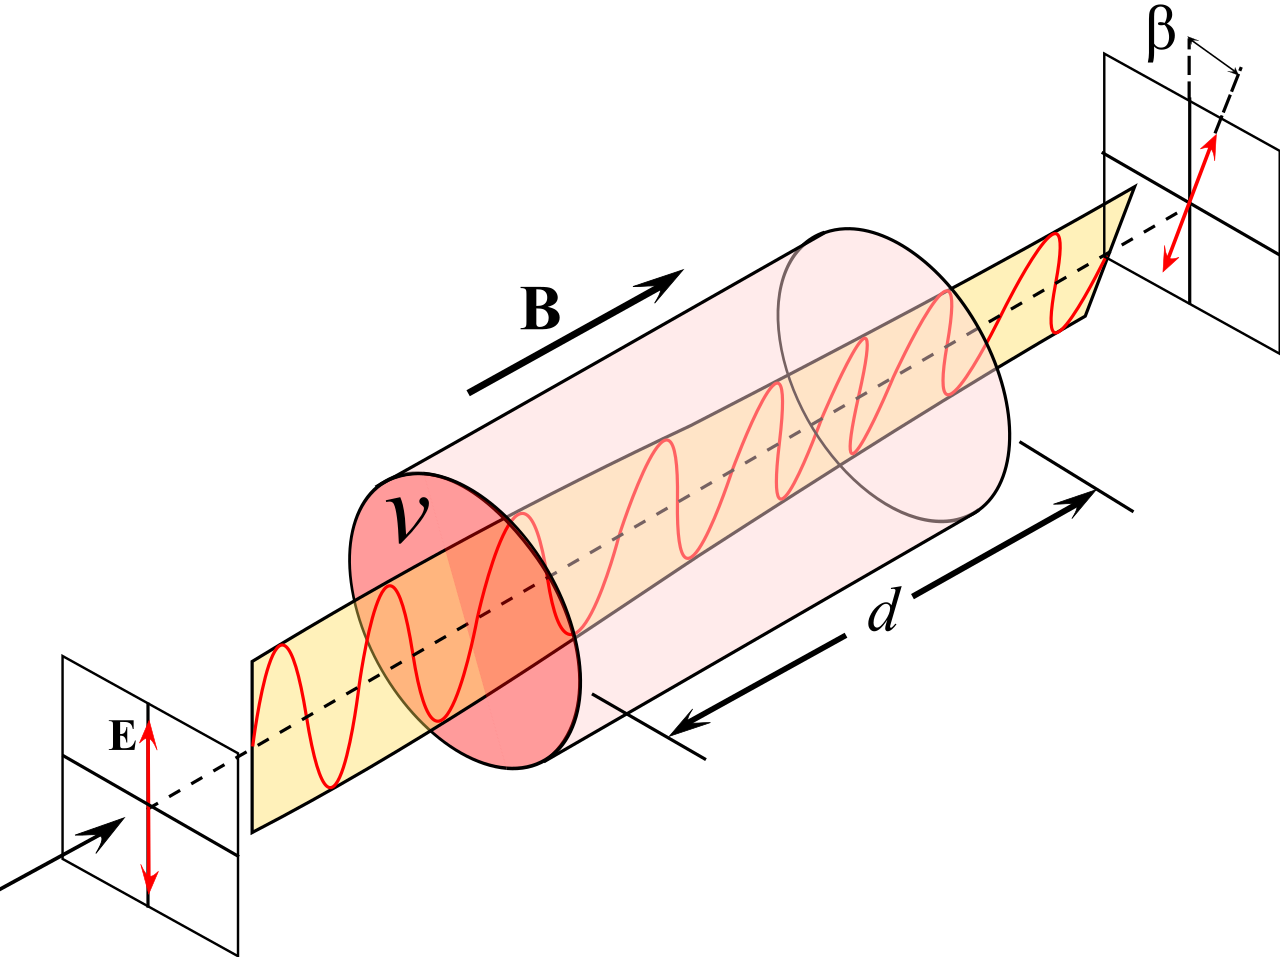
\includegraphics[scale=0.1]{images/faraday.png}\\[-1.5\baselineskip]%
                \hspace{1.5cm}{[JunCTionS, Wikipedia]}}%
            \only <3>{%
                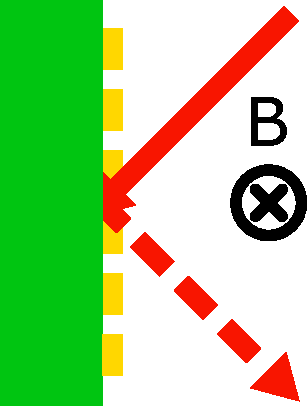
\includegraphics[scale=0.4]{images/TMOKE.pdf}\\[-0.5\baselineskip]%
                \hspace{1.5cm}{[Lars Klompmaker, Masterarbeit]}}%
            \only <4->{%
                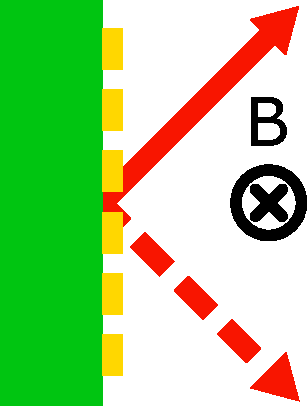
\includegraphics[scale=0.4]{images/TMRLE.pdf}\\[-0.5\baselineskip]%
                \hspace{1.5cm}{[Lars Klompmaker, Masterarbeit]}}%      
        \end{column}
    \end{columns}
\end{frame}